% ============================================================
%  RAPPORT DE SOUTENANCE — MOBIUS ROGUELIKE
%  M3G_STUDIO — Projet Jeu-Vidéo EPITA 2025-2026
% ============================================================
\documentclass[12pt,a4paper]{article}
\usepackage[utf8]{inputenc}
\usepackage[T1]{fontenc}
\usepackage{graphicx}
\usepackage{url}

% Configuration des liens sans couleur ni bordure
\usepackage[hidelinks]{hyperref}

% Marges
\usepackage[margin=2.5cm]{geometry}

% Espacement entre les lignes
\usepackage{setspace}

% ── Packages supplémentaires ───────────────────────────────
% \usepackage[french]{babel} % non disponible dans cet environnement
\usepackage{xcolor}
\usepackage{float}
\usepackage{caption}
\usepackage{subcaption}
\usepackage{booktabs}
\usepackage{array}
\usepackage{tabularx}
\usepackage{multirow}
\usepackage{enumitem}
\usepackage{listings}
\usepackage{fancyhdr}
\usepackage{lastpage}
\usepackage{titlesec}
\usepackage{tocloft}
\usepackage{parskip}
\usepackage{mdframed}
\usepackage{amssymb}
\usepackage{colortbl}

% ╔══════════════════════════════════════════════════════════╗
%  PALETTE DE COULEURS
% ╚══════════════════════════════════════════════════════════╝
\definecolor{titlegray}{RGB}{20,20,20}
\definecolor{sectionblue}{RGB}{25,60,120}
\definecolor{rulegray}{RGB}{140,140,140}
\definecolor{lightbg}{RGB}{248,249,252}
\definecolor{framegray}{RGB}{200,200,200}
\definecolor{okgreen}{RGB}{20,120,20}
\definecolor{warnorange}{RGB}{170,90,0}
\definecolor{codelisting}{RGB}{245,246,250}
\definecolor{accentblue}{RGB}{30,80,160}
\definecolor{tableheadbg}{RGB}{230,235,245}
\definecolor{rowaltbg}{RGB}{250,251,254}

% ╔══════════════════════════════════════════════════════════╗
%  ESPACEMENT
% ╚══════════════════════════════════════════════════════════╝
\onehalfspacing
\setlength{\parindent}{0pt}
\setlength{\parskip}{6pt plus 2pt minus 1pt}

% ╔══════════════════════════════════════════════════════════╗
%  STYLE DES TITRES DE SECTIONS
% ╚══════════════════════════════════════════════════════════╝
\titleformat{\section}
  {\normalfont\Large\bfseries\color{sectionblue}}
  {\thesection}{0.8em}{}
  [\vspace{2pt}{\color{rulegray}\hrule height 0.6pt}\vspace{4pt}]

\titleformat{\subsection}
  {\normalfont\large\bfseries\color{titlegray}}
  {\thesubsection}{0.7em}{}

\titleformat{\subsubsection}
  {\normalfont\normalsize\bfseries\itshape\color{titlegray}}
  {\thesubsubsection}{0.6em}{}

\titlespacing*{\section}{0pt}{18pt}{8pt}
\titlespacing*{\subsection}{0pt}{12pt}{4pt}

% ╔══════════════════════════════════════════════════════════╗
%  EN-TÊTES / PIEDS DE PAGE
% ╚══════════════════════════════════════════════════════════╝
\pagestyle{fancy}
\fancyhf{}
\fancyhead[L]{\small\textbf{\textcolor{sectionblue}{MOBIUS} Roguelike} \textemdash{} M3G\_STUDIO}
\fancyhead[R]{\small\textcolor{gray}{Rapport de soutenance \textemdash{} EPITA 2026}}
\fancyfoot[C]{\small\thepage\ / \pageref{LastPage}}
\renewcommand{\headrulewidth}{0.5pt}
\renewcommand{\footrulewidth}{0.2pt}
\setlength{\headheight}{15pt}

% ╔══════════════════════════════════════════════════════════╗
%  STYLE DE CODE
% ╚══════════════════════════════════════════════════════════╝
\lstset{
  language=Python,
  basicstyle=\ttfamily\small,
  keywordstyle=\bfseries\color{sectionblue},
  stringstyle=\color{gray},
  commentstyle=\color{gray}\itshape,
  backgroundcolor=\color{codelisting},
  frame=single,
  rulecolor=\color{framegray},
  breaklines=true,
  showstringspaces=false,
  numbers=left,
  numberstyle=\tiny\color{gray},
  numbersep=6pt,
  xleftmargin=16pt,
  captionpos=b,
}

% ╔══════════════════════════════════════════════════════════╗
%  BOÎTE INFO
% ╚══════════════════════════════════════════════════════════╝
\newmdenv[
  linecolor=sectionblue,
  linewidth=1.2pt,
  backgroundcolor=lightbg,
  innerleftmargin=12pt,
  innerrightmargin=12pt,
  innertopmargin=10pt,
  innerbottommargin=10pt,
  roundcorner=4pt,
]{infobox}

% ── Commande pour les cases à cocher ──────────────────────
\newcommand{\okitem}{\textcolor{okgreen}{$\checkmark$}}
\newcommand{\warnitem}{\textcolor{warnorange}{$\sim$}}

% ── Commande titre de section avec badge ──────────────────
\newcommand{\member}[2]{%
  \noindent\textbf{#1}\quad{\small\textcolor{gray}{#2}}%
}

% ============================================================
\begin{document}

% ╔══════════════════════════════════════════════════════════╗
%  PAGE DE TITRE
% ╚══════════════════════════════════════════════════════════╝
\begin{titlepage}
  \centering
  \vspace*{1.5cm}

  % Logo (à décommenter si disponible)
  % 
\includegraphics[width=0.42\textwidth]{mobius_logo_final.png}\\[1.2cm]

  {\color{rulegray}\rule{12cm}{0.5pt}}\\[0.5cm]

  {\LARGE\bfseries\color{titlegray} MOBIUS}\\[0.3cm]
  {\large\bfseries\color{sectionblue} R O G U E L I K E}\\[0.4cm]

  {\color{rulegray}\rule{12cm}{0.5pt}}\\[1.2cm]

  {\large\bfseries Rapport de soutenance \textemdash{} Projet Jeu-Vidéo}\\[0.4cm]
  {\normalsize\color{gray}EPITA \textemdash{} Promo 2030 \textemdash{} Soutenance du 27 mars 2026}\\[2cm]

  \begin{mdframed}[
    linecolor=sectionblue,
    linewidth=1.5pt,
    innerleftmargin=20pt,
    innerrightmargin=20pt,
    innertopmargin=14pt,
    innerbottommargin=14pt,
    roundcorner=4pt,
  ]
  \centering
  {\Large\bfseries M3G\_STUDIO}\\[4pt]
  {\small\color{gray} Studio de développement indépendant}
  \end{mdframed}

  \vspace{2cm}

  \begin{tabular}{@{}ll@{}}
    \textbf{Georges Boyer}         & Chef de groupe \textemdash{} Développement principal \\[6pt]
    \textbf{Madeleine Diop}        & Environnement visuel \& graphismes \\[6pt]
    \textbf{Emile Levast}          & Lore, narration \& site web \\[6pt]
    \textbf{Maël Bosse-Platière}   & Multijoueur en ligne \\
  \end{tabular}

  \vfill
  {\small\color{gray} 27 mars 2026}
\end{titlepage}

% ╔══════════════════════════════════════════════════════════╗
%  TABLE DES MATIÈRES
% ╚══════════════════════════════════════════════════════════╝
\tableofcontents
\newpage

% ============================================================
\section{Introduction}

Ce rapport de soutenance présente l'avancement du projet \textbf{MOBIUS Roguelike}, réalisé dans le cadre du projet \textit{Jeu-Vidéo} de première année à l'EPITA (promo 2030). Il retrace les choix techniques et créatifs effectués par l'équipe M3G\_STUDIO, les fonctionnalités implémentées, ainsi que le bilan organisationnel du groupe.

% ─────────────────────────────────────────────────────────────
\subsection{Présentation du projet}

MOBIUS est un jeu de type \textit{roguelike} en vue du dessus (\textit{top-down shooter}) développé entièrement en Python avec la bibliothèque Pygame. Le principe central est un voyage à travers six époques historiques : le joueur affronte des vagues d'ennemis propres à chaque ère, récupère des armes dans des coffres, et tente de survivre jusqu'à l'ère Futuriste.

Le jeu propose deux modes : un mode \textbf{solo} et un mode \textbf{multijoueur en ligne} (co-op 2 joueurs via UDP), chacun supportant la sélection d'une classe de personnage parmi cinq disponibles.

\begin{infobox}
\textbf{Fiche technique}\\[6pt]
\begin{tabular}{@{}ll@{}}
  \textbf{Moteur / Langage} & Python 3.11+ / Pygame 2.x \\[2pt]
  \textbf{Résolution}       & Plein écran adaptatif (détection dynamique) \\[2pt]
  \textbf{Réseau}           & UDP maison, port 55\,555, architecture client-serveur \\[2pt]
  \textbf{Époques}          & 6 : Préhistoire $\to$ Grèce $\to$ Edo $\to$ Moderne $\to$ WW2 $\to$ Futur \\[2pt]
  \textbf{Classes}          & 5 : Tank, Berserker, Vampire, Ninja, Archer \\[2pt]
  \textbf{Armes}            & Distanciel, mêlée, AOE selon l'époque \\
\end{tabular}
\end{infobox}

% ─────────────────────────────────────────────────────────────
\subsection{Présentation du groupe}

Notre groupe M3G\_STUDIO est composé de quatre étudiants en première année à l'EPITA (promo 2030), réunis autour d'une passion commune pour les jeux vidéo et la programmation.

\subsubsection*{Georges Boyer \textemdash{} Chef de groupe, développement principal}

Passionné de programmation, Georges a naturellement pris en charge l'architecture générale du projet. Il a conçu le moteur de jeu (\texttt{base\_room.py}), l'orchestrateur principal (\texttt{main.py}), le système de mécaniques (\texttt{mechanics.py}) et les constantes globales (\texttt{constants.py}). En tant que chef de groupe, il a également coordonné les réunions d'avancement et l'intégration des différents modules.

\subsubsection*{Madeleine Diop \textemdash{} Environnement visuel \& graphismes}

Madeleine a pris en charge tout le rendu visuel du jeu : création des fonds thématiques par époque, effets de particules (pétales de cerisier dans l'ère Edo, pluie WW2, fumée napoléonienne, scan holographique futuriste), et cohérence graphique globale. Elle a développé le module \texttt{graphics.py} comprenant le \texttt{SpriteCache}, le \texttt{BackgroundRenderer} et les \texttt{ScreenEffects}.

\begin{mdframed}[
  linecolor=rulegray,
  linewidth=0.8pt,
  backgroundcolor=rowaltbg,
  innerleftmargin=10pt,
  innerrightmargin=10pt,
  innertopmargin=6pt,
  innerbottommargin=6pt,
  roundcorner=3pt,
]
\textit{``Rendre chaque époque unique visuellement sans alourdir les performances a été mon défi principal. Les effets de particules différenciés par époque ont vraiment enrichi l'immersion.''}
\end{mdframed}

\subsubsection*{Emile Levast \textemdash{} Lore, narration \& site web}

Emile s'est chargé de l'univers narratif du jeu et de la communication externe. Il a défini le \textit{lore} de MOBIUS (l'histoire du voyageur temporel, la logique des six époques), rédigé les textes du jeu, et développé le site web de M3G\_STUDIO.

\subsubsection*{Maël Bosse-Platière \textemdash{} Multijoueur en ligne}

Maël a développé le module réseau complet du jeu (\texttt{network.py}). Il a implémenté une architecture client-serveur UDP maison : le \texttt{GameServer} joue le rôle de serveur autoritaire, le \texttt{GameClient} envoie ses inputs et reçoit l'état du jeu pour l'afficher via le \texttt{ClientRenderer}.

% ─────────────────────────────────────────────────────────────
\subsection{But du projet}

\subsubsection*{Origine}

M3G\_STUDIO est né de la volonté de créer un jeu original qui dépasse le simple exercice scolaire. L'idée centrale --- traverser les grandes époques de l'humanité en affrontant des ennemis historiques --- est née d'une réflexion sur ce qui rend un roguelike rejouable : la variation. En changeant radicalement d'univers visuel, d'armes et d'ennemis à chaque époque, chaque \textit{run} offre une expérience différente.

\subsubsection*{Nature du jeu}

MOBIUS est un \textit{top-down shooter roguelike} : le joueur évolue dans des arènes en vue aérienne, élimine des vagues d'ennemis de difficulté croissante, et récupère des améliorations (\textit{power-ups}) et armes dans des coffres. La mécanique de progression par époques --- chacune avec ses propres ennemis, armes et ambiance visuelle --- est le fil conducteur du jeu.

\subsubsection*{Objectif}

Livrer un jeu jouable, complet et soigné : menus animés, sélection de classe, six époques jouables, mode solo et multijoueur en ligne, et un rendu visuel cohérent avec l'identité de M3G\_STUDIO.

% ─────────────────────────────────────────────────────────────
\subsection{Présentation de l'entreprise fictive}

\textbf{M3G\_STUDIO} a été fondé pour ce projet par les quatre membres de l'équipe. Le nom reprend les initiales des fondateurs et affirme une identité collective. Notre studio se spécialise dans les jeux indépendants à fort caractère narratif et visuel, en particulier les roguelikes et les jeux d'action à progression.

Notre premier titre, \textbf{MOBIUS Roguelike}, illustre notre philosophie : un gameplay accessible mais profond, une direction artistique soignée, et une rejouabilité portée par la variation des univers.

% ─────────────────────────────────────────────────────────────
\subsection{État de l'art \& inspirations}

Le genre roguelike top-down est largement représenté dans l'industrie indépendante. Parmi les titres de référence :

\begin{itemize}[noitemsep, leftmargin=1.5em]
  \item \textbf{Enter the Gungeon} (Dodge Roll, 2016) : référence du top-down shooter roguelike avec progression par armes.
  \item \textbf{Hades} (Supergiant Games, 2020) : roguelike narratif avec runs courts et progression méta.
  \item \textbf{Nuclear Throne} (Vlambeer, 2015) : roguelike action intense avec personnages aux capacités distinctes.
  \item \textbf{Vampire Survivors} (poncle, 2022) : popularisation du \textit{bullet heaven} avec progression automatique.
  \item \textbf{Call of Duty Zombies} (Treyarch, 2008) : inspiration pour le système de vagues d'ennemis croissantes.
\end{itemize}

MOBIUS se différencie par son système d'époques historiques qui transforme radicalement l'ambiance et les mécaniques à chaque niveau, et par son mode co-op en ligne intégré. \textbf{Enter the Gungeon} a directement inspiré notre système d'armes variées et la mécanique de coffres. La sélection de classe s'inspire de \textbf{Hades}. La progression en vagues s'inspire de \textbf{Vampire Survivors} et de \textbf{Call of Duty Zombies}.

% ─────────────────────────────────────────────────────────────
\subsection{Répartition des tâches}

\begin{table}[H]
\centering
\caption{Répartition des tâches par membre}
\renewcommand{\arraystretch}{1.4}
\begin{tabularx}{\textwidth}{@{}>{\bfseries}lXc@{}}
\toprule
\rowcolor{tableheadbg}
\textbf{Membre} & \textbf{Périmètre} & \textbf{État} \\
\midrule
Georges Boyer       & Architecture (base\_room, main, mechanics, constants), IA ennemis, système d'armes, classes joueur, coffres, power-ups & \textcolor{warnorange}{\textbf{En cours}} \\
\rowcolor{rowaltbg}
Madeleine Diop      & Graphismes (graphics.py), effets par époque, backgrounds, HUD, sprites & \textcolor{warnorange}{\textbf{En cours}} \\
Emile Levast        & Lore des époques, textes in-game, site web M3G\_STUDIO & \textcolor{okgreen}{\textbf{Terminé}} \\
\rowcolor{rowaltbg}
Maël Bosse-Platière & Module réseau UDP (network.py), synchronisation client-serveur, gestion déconnexion & \textcolor{warnorange}{\textbf{En cours}} \\
\bottomrule
\end{tabularx}
\end{table}

% ─────────────────────────────────────────────────────────────
\subsection{Ressenti global du projet}

Le développement de MOBIUS a été une expérience intense et formatrice. Partir d'une idée et aboutir à un jeu fonctionnel avec menu, multijoueur, six univers distincts et un système de classes en quelques semaines nous a confrontés à des défis bien au-delà du simple cours de Python. Les difficultés ont été nombreuses --- synchronisation réseau, gestion des ressources visuelles, cohérence des états du jeu --- mais chaque obstacle résolu a renforcé notre maîtrise des outils et notre dynamique d'équipe.

% ============================================================
\newpage
\section{Avancement du projet}

% ─────────────────────────────────────────────────────────────
\subsection{Scénario et univers}

\subsubsection*{Contexte narratif}

Le joueur incarne un voyageur temporel coincé dans une boucle infinie --- une \textit{bande de Möbius} --- qui le fait traverser six époques de l'histoire humaine. À chaque époque, des créatures hostiles ont envahi la ligne temporelle et menacent l'intégrité du continuum. Le joueur doit les éliminer pour passer à l'époque suivante, en s'adaptant aux armes et aux techniques de combat propres à chaque ère.

\subsubsection*{Progression par époques}

\begin{table}[H]
\centering
\caption{Époques, thèmes et multiplicateurs de difficulté}
\renewcommand{\arraystretch}{1.35}
\begin{tabular}{@{}clcc@{}}
\toprule
\rowcolor{tableheadbg}
\textbf{Ordre} & \textbf{Époque} & \textbf{Difficulté} & \textbf{Ambiance} \\
\midrule
1 & Préhistoire     & $\times 1.0$ & Âge de pierre, cavernes, feux de camp \\
\rowcolor{rowaltbg}
2 & Grèce Antique   & $\times 1.3$ & Temples, Olympe, soleil méditerranéen \\
3 & Période Edo     & $\times 1.6$ & Japon médiéval, cerisiers, nuit étoilée \\
\rowcolor{rowaltbg}
4 & Ère Moderne     & $\times 2.0$ & Napoléon, champs de bataille, fumée de canon \\
5 & Guerre Mondiale & $\times 2.5$ & WW2, jungle, bunker, pluie \\
\rowcolor{rowaltbg}
6 & Ère Futuriste   & $\times 3.0$ & Station spatiale, néons, hologrammes \\
\bottomrule
\end{tabular}
\end{table}

\subsubsection*{Transitions entre époques}

Les transitions sont gérées par la classe \texttt{EpochTransition} dans \texttt{main.py} : un fondu noir progressif accompagné du nom de l'époque en grand texte. La progression des stats du joueur (PV, stamina, kills, coins) est conservée entre les époques.

% ─────────────────────────────────────────────────────────────
\subsection{Mécaniques de jeu}

\subsubsection*{Déplacements du joueur}

Le joueur se déplace au clavier (ZQSD) et vise à la souris. Un système de \textbf{dash} (touche \texttt{ESPACE}) permet une esquive rapide avec cooldown (\texttt{DASH\_COOLDOWN = 30} frames) et coût en stamina (\texttt{DASH\_STAMINA\_COST = 15}). La vitesse de base est modulée par la classe choisie.

\subsubsection*{Système d'armes}

Les armes sont définies dans \texttt{WEAPONS\_DATA} et instanciées via la classe \texttt{Weapon}. Chaque arme possède :
\begin{itemize}[noitemsep, leftmargin=1.5em]
  \item Un type (\texttt{ranged} ou \texttt{melee})
  \item Des dégâts (\texttt{damage}), un cooldown (\texttt{cooldown\_max}) et un coût en stamina
  \item Pour les armes à distance : vitesse de projectile (\texttt{projectile\_speed})
  \item Pour la mêlée : portée d'arc d'attaque (\texttt{melee\_range})
\end{itemize}

Les projectiles joueur (\texttt{Bullet}) héritent du sprite de l'arme, rotationné selon la direction de tir. Les attaques de mêlée (\texttt{MeleeAttack}) génèrent une ellipse d'arc positionnée dans la direction visée.

\subsubsection*{Classes de personnage}

\begin{table}[H]
\centering
\caption{Classes disponibles et leurs caractéristiques}
\renewcommand{\arraystretch}{1.35}
\begin{tabular}{@{}lll@{}}
\toprule
\rowcolor{tableheadbg}
\textbf{Classe} & \textbf{Stats} & \textbf{Compétence spéciale} \\
\midrule
Tank       & 150 PV, Vitesse $-30\%$ & Bouclier : $-50\%$ dégâts reçus \\
\rowcolor{rowaltbg}
Berserker  & 80 PV, Vitesse $+30\%$  & Rage : $\times 2$ dégâts pendant 5s \\
Vampire    & Stats normales           & $+10$ PV par kill (10s) \\
\rowcolor{rowaltbg}
Ninja      & PV réduits, Vitesse max  & Invisibilité brève \\
Archer     & Stats normales           & Flèche multiple à distance \\
\bottomrule
\end{tabular}
\end{table}

\subsubsection*{Power-ups et coffres}

Les \textbf{power-ups} (classe \texttt{PowerUp}) apparaissent aléatoirement et offrent quatre types de bonus : \textit{Damage}, \textit{Speed}, \textit{Health}, \textit{Stamina}. Ils pulsent visuellement et disparaissent après 600 frames s'ils ne sont pas ramassés.

Les \textbf{coffres} (classe \texttt{Chest}) contiennent une arme spécifique à l'époque. Le joueur les ouvre en s'approchant (touche \texttt{E}), déclenchant une animation d'ouverture et l'ajout de l'arme à son inventaire.

% ─────────────────────────────────────────────────────────────
\subsection{Fonctionnalités}

\subsubsection*{Menu principal \& navigation}

Le menu principal (\texttt{MainMenuRenderer}) affiche le logo MOBIUS avec une animation flottante, des particules de fond et deux boutons : \textit{Jouer} et \textit{Quitter}. L'écran de mode (\texttt{ModeSelectRenderer}) présente deux grandes cartes cliquables --- \textbf{Solo} et \textbf{En ligne} --- avec effets de survol animés. Un slider de volume persistant (\texttt{VolumeSlider}) est présent sur tous les écrans de menus.

\begin{figure}[H]
  \centering
  \caption{ref annexe: Écran titre \textemdash{} Menu principal MOBIUS}
\end{figure}

\subsubsection*{Sélection de classe}

L'écran \texttt{MenuRenderer} affiche cinq cartes de classe avec dégradé de couleur, icône, description et compétence spéciale. Un effet de surbrillance et d'élévation indique la carte survolée. La sélection se fait au clic ou via les touches \texttt{1}--\texttt{5}.

\subsubsection*{HUD (affichage tête haute)}

Le HUD affiche en temps réel : barre de PV, barre de stamina, arme courante avec cooldown visuel, nom de l'époque, numéro de vague, compteur de kills et de pièces collectées, et indicateur de compétence spéciale.

\begin{figure}[H]
  \centering
  \caption{ref annexe: HUD pendant une partie}
\end{figure}

% ─────────────────────────────────────────────────────────────
\subsection{Multijoueur en ligne}
\label{sec:multi}

\subsubsection*{Architecture réseau}

Le module \texttt{network.py} implémente une architecture \textbf{client-serveur autoritaire sur UDP} (port 55\,555 par défaut). Le \textbf{HOST} est le serveur : il simule l'intégralité du jeu et envoie l'état complet au client à chaque frame. Le \textbf{CLIENT} n'effectue aucune simulation locale : il envoie ses inputs (déplacement, tir, dash\ldots) et reçoit l'état du jeu via le \texttt{ClientRenderer}.

\subsubsection*{Flux de connexion}

\begin{enumerate}[noitemsep, leftmargin=1.8em]
  \item Le HOST lance le serveur UDP et attend le client (écran \textit{En attente de P2\ldots}).
  \item Le CLIENT saisit l'IP du host (\texttt{IPInputRenderer}) et se connecte dans un thread séparé pour ne pas bloquer l'UI.
  \item Une fois connectés, chaque joueur arrive sur l'écran de sélection de classe.
  \item Le HOST envoie le signal \texttt{send\_start} ; le jeu démarre simultanément.
\end{enumerate}

\subsubsection*{Synchronisation}

Éléments synchronisés à chaque frame :
\begin{itemize}[noitemsep, leftmargin=1.5em]
  \item Position et direction du joueur P2
  \item Points de vie de P2
  \item État des ennemis (position, PV)
  \item Projectiles ennemis actifs
  \item Transitions d'époques et événements \textit{game-over}
\end{itemize}

La gestion des timeouts (8 secondes) permet de détecter proprement une déconnexion.

\subsubsection*{Défis rencontrés}

L'implémentation réseau a posé plusieurs problèmes techniques : la sérialisation efficace de l'état du jeu (nombreux sprites), la gestion de la latence variable en UDP, et la synchronisation des transitions d'époque entre les deux machines. La solution retenue --- serveur autoritaire sans prédiction client --- privilégie la simplicité et la cohérence.

% ─────────────────────────────────────────────────────────────
\subsection{Graphismes et environnement visuel}

\subsubsection*{Décors par époque}

Chaque époque dispose d'une classe héritant de \texttt{BaseRoom} et implémentant \texttt{draw\_epoch\_decoration()} :

\begin{table}[H]
\centering
\caption{Effets visuels par époque}
\renewcommand{\arraystretch}{1.35}
\begin{tabular}{@{}lll@{}}
\toprule
\rowcolor{tableheadbg}
\textbf{Époque} & \textbf{Couleur thématique} & \textbf{Effet de décoration} \\
\midrule
Préhistoire      & Brun (139, 69, 19)      & Flammes animées (optionnelles) \\
\rowcolor{rowaltbg}
Grèce Antique    & Or grec (200, 180, 80)  & Soleil animé (optionnel) \\
Période Edo      & Rouge (180, 30, 30)     & Pétales de cerisier flottants \\
\rowcolor{rowaltbg}
Ère Moderne      & Bleu (0, 80, 160)       & Volutes de fumée de canon \\
Guerre Mondiale  & Vert (60, 80, 40)       & Pluie battante \\
\rowcolor{rowaltbg}
Ère Futuriste    & Cyan (0, 220, 255)      & Scan holographique + chiffres 0/1 \\
\bottomrule
\end{tabular}
\end{table}

\subsubsection*{Système de sprites et cache}

Le module \texttt{graphics.py} centralise le chargement des assets via la classe \texttt{SpriteCache} (singleton) qui évite les rechargements redondants. Le \texttt{BackgroundRenderer} génère les fonds thématiques par époque. Les \texttt{ScreenEffects} gèrent les flashs d'impact, les fades et les effets de transition.

\begin{figure}[H]
  \centering
  \begin{subfigure}[b]{0.47\textwidth}
    \caption{ref annexe: Ère Edo}
  \end{subfigure}
  \hfill
  \begin{subfigure}[b]{0.47\textwidth}
    \caption{ref annexe: Ère Futuriste}
  \end{subfigure}
  \caption{ref annexe: Exemples de décorations d'époque}
\end{figure}

% ─────────────────────────────────────────────────────────────
\subsection{Architecture du code}

\subsubsection*{Structure modulaire}

\begin{mdframed}[
  linecolor=framegray,
  linewidth=0.8pt,
  backgroundcolor=codelisting,
  innerleftmargin=12pt,
  innerrightmargin=12pt,
  innertopmargin=8pt,
  innerbottommargin=8pt,
]
\begin{verbatim}
mobius/
|-- main.py               # Orchestrateur, etats, menus, boucle principale
|-- core/
|   |-- constants.py      # Couleurs, donnees armes, skills, epochs
|   |-- graphics.py       # SpriteCache, BackgroundRenderer, ScreenEffects
|   |-- mechanics.py      # Weapon, Bullet, MeleeAttack, PowerUp, Chest
|   |-- base_room.py      # Classe mere de toutes les salles
|   `-- network.py        # GameServer, GameClient, ClientRenderer
`-- epoques/
    |-- prehistoire.py    # Salle ere Prehistorique
    |-- grece.py          # Salle Grece Antique
    |-- edo.py            # Salle Periode Edo
    |-- moderne.py        # Salle Ere Moderne
    |-- contemporain.py   # Salle Guerre Mondiale
    `-- futuristique.py   # Salle Ere Futuriste
\end{verbatim}
\end{mdframed}

\subsubsection*{Machine à états}

La classe \texttt{Game} gère l'état global du jeu via des constantes entières :

\begin{table}[H]
\centering
\caption{États du jeu et transitions}
\renewcommand{\arraystretch}{1.35}
\begin{tabular}{@{}lll@{}}
\toprule
\rowcolor{tableheadbg}
\textbf{État} & \textbf{Description} & \textbf{Transition vers} \\
\midrule
\texttt{MAIN\_MENU}        & Écran titre          & \texttt{MODE\_SELECT} \\
\rowcolor{rowaltbg}
\texttt{MODE\_SELECT}      & Solo ou En ligne     & \texttt{CHARACTER\_SELECT} / \texttt{ONLINE\_MENU} \\
\texttt{ONLINE\_MENU}      & Héberger / Rejoindre & \texttt{WAITING\_CLIENT} / \texttt{IP\_INPUT} \\
\rowcolor{rowaltbg}
\texttt{CHARACTER\_SELECT} & Choix de classe      & \texttt{PLAYING} \\
\texttt{PLAYING}           & Jeu en cours         & \texttt{GAME\_OVER} \\
\rowcolor{rowaltbg}
\texttt{GAME\_OVER}        & Fin de partie        & \texttt{MAIN\_MENU} / \texttt{PLAYING} \\
\bottomrule
\end{tabular}
\end{table}

\subsubsection*{Extrait de code représentatif}

\begin{lstlisting}[caption={Méthode \texttt{change\_epoch()} dans \texttt{main.py} \textemdash{} transition d'époque avec persistance des stats}]
def change_epoch(self, next_epoch: str | None):
    if next_epoch and next_epoch in self.rooms:
        p = self.current_room.player
        stats = {"skill": p.skill, "kills": p.kills,
                 "coins": p.coins, "health": p.health,
                 "max_health": p.max_health}
        def _do():
            self.current_epoch = next_epoch
            self.current_room  = self.rooms[next_epoch]
            self.current_room.start(
                stats["skill"], mode=self.net_mode,
                player_stats=stats, server=self.server)
            if self.server:
                self.server.send_start(stats["skill"])
        self.transition.start(next_epoch, _do)
    else:
        self.game_state = GAME_OVER
\end{lstlisting}

% ============================================================
\newpage
\section{Bilan de l'avancement}

\subsection{Ce qui a été réalisé}

L'ensemble des fonctionnalités prévues en priorité haute a été livré :

\begin{itemize}[leftmargin=1.8em, itemsep=2pt]
  \item[\okitem] Six époques jouables avec décors distincts, ennemis et armes thématiques
  \item[\okitem] Cinq classes de personnage avec compétences spéciales
  \item[\okitem] Système d'armes complet (distanciel, mêlée, projectiles ennemis)
  \item[\okitem] Coffres et power-ups avec animations
  \item[\okitem] Menus animés complets (titre, mode, classe, game over)
  \item[\okitem] Transitions d'époques avec fondu et texte animé
  \item[\okitem] Mode solo pleinement fonctionnel
  \item[\okitem] Module réseau UDP avec architecture client-serveur
  \item[\okitem] HUD complet (PV, stamina, arme, vague, kills, coins)
  \item[\okitem] Logo et identité visuelle M3G\_STUDIO
  \item[\okitem] Site web M3G\_STUDIO (Emile Levast)
\end{itemize}

\subsection{Difficultés et ajustements}

\begin{itemize}[leftmargin=1.5em, itemsep=4pt]
  \item \textbf{Flammes préhistoriques et soleil grec} : ces effets ont été désactivés pour raisons de performance. Ils restent commentés dans le code et sont réactivables facilement.
  \item \textbf{Synchronisation réseau complète} : le rendu client est fonctionnel mais certains effets de particules ne sont pas transmis. La synchronisation des sons reste partielle.
  \item \textbf{Mode LAN vs Internet} : le multijoueur fonctionne de façon fiable en réseau local. Sur Internet, l'ouverture du port UDP 55\,555 reste nécessaire côté hôte.
\end{itemize}

\subsection{Écarts prévisionnel / réel}

\begin{table}[H]
\centering
\caption{Comparaison prévisionnel vs réalisé}
\renewcommand{\arraystretch}{1.4}
\begin{tabularx}{\textwidth}{@{}Xcc@{}}
\toprule
\rowcolor{tableheadbg}
\textbf{Fonctionnalité} & \textbf{Prévu} & \textbf{Réalisé} \\
\midrule
6 époques jouables            & Oui   & \textcolor{okgreen}{\textbf{Oui}} \\
\rowcolor{rowaltbg}
5 classes joueur              & Oui   & \textcolor{okgreen}{\textbf{Oui}} \\
Mode solo                     & Oui   & \textcolor{okgreen}{\textbf{Oui}} \\
\rowcolor{rowaltbg}
Mode multijoueur LAN          & Oui   & \textcolor{okgreen}{\textbf{Oui}} \\
Mode multijoueur Internet     & Oui   & \textcolor{warnorange}{\textbf{Partiel}} \\
\rowcolor{rowaltbg}
Effets décor toutes époques   & Oui   & \textcolor{warnorange}{\textbf{4/6 actifs}} \\
Site web M3G\_STUDIO          & Oui   & \textcolor{okgreen}{\textbf{Oui}} \\
\rowcolor{rowaltbg}
Sons / Musique                & Bonus & \textcolor{warnorange}{\textbf{Partiel}} \\
\bottomrule
\end{tabularx}
\end{table}

% ============================================================
\newpage
\section{Communication}

\subsection{Site web M3G\_STUDIO}

Le site web de M3G\_STUDIO a été réalisé par Emile Levast. Il présente le studio, le jeu MOBIUS, les membres de l'équipe, et propose un lien de téléchargement du jeu. Le site reflète l'identité visuelle de MOBIUS et inclut des pages dédiées au lore des six époques et aux contrôles du jeu.

\begin{figure}[H]
  \centering
  \caption{ref annexe: Site web M3G\_STUDIO}
\end{figure}

\subsection{Logo et identité visuelle}

Le logo MOBIUS a été conçu en pixel-art avec un dégradé cyan vers bleu profond, agrémenté d'un effet de foudre rose en bas. Ce logo est utilisé de façon cohérente sur l'écran titre, dans tous les menus, sur le site web et dans les documents du projet.

% \begin{figure}[H]
%   \centering
%   
\includegraphics[width=0.38\textwidth]{mobius_logo_final.png}
%   \caption{Logo officiel MOBIUS \textemdash{} M3G\_STUDIO}
% \end{figure}

\subsection{Manuel d'utilisation}

Les contrôles du jeu sont affichés directement dans l'interface de sélection de mode, garantissant que le joueur est informé avant de commencer.

\begin{table}[H]
\centering
\caption{Contrôles du jeu}
\renewcommand{\arraystretch}{1.35}
\begin{tabular}{@{}ll@{}}
\toprule
\rowcolor{tableheadbg}
\textbf{Touche} & \textbf{Action} \\
\midrule
\texttt{ZQSD}        & Déplacement \\
\rowcolor{rowaltbg}
\texttt{Clic gauche} & Tirer / Attaquer \\
\texttt{ESPACE}      & Dash (esquive) \\
\rowcolor{rowaltbg}
\texttt{F}           & Compétence spéciale \\
\texttt{E}           & Ouvrir un coffre \\
\rowcolor{rowaltbg}
\texttt{1 / 2}       & Changer d'arme \\
\texttt{ESC}         & Menu pause / Retour \\
\bottomrule
\end{tabular}
\end{table}

% ============================================================
\newpage
\section{Conclusion}

Le développement de MOBIUS Roguelike a représenté pour M3G\_STUDIO bien plus qu'un exercice académique. En partant de zéro pour concevoir un jeu complet --- architecture modulaire, graphismes thématiques, système de classes, et multijoueur en ligne --- nous avons collectivement franchi un cap significatif dans notre maîtrise de Python et de la conception logicielle.

Le résultat est un jeu jouable, cohérent visuellement et narrativement, avec une rejouabilité portée par les six univers distincts et les cinq classes. Le module réseau UDP, développé sans framework, constitue techniquement la partie la plus ambitieuse du projet.

Ce que ce projet nous a appris dépasse le code : planification réaliste, communication régulière, gestion des imprévus, et fierté collective d'un livrable abouti. Ces compétences nous accompagneront bien au-delà de la promo 2030.

\vspace{1.5cm}
\begin{center}
  {\large\bfseries M3G\_STUDIO \textemdash{} MOBIUS Roguelike \textemdash{} EPITA 2026}\\[8pt]
  {\color{gray}\rule{8cm}{0.4pt}}\\[6pt]
  \textit{``Every loop ends. Until it doesn't.''}
\end{center}

% ============================================================
%  ANNEXES
% ============================================================
\newpage
\appendix
\renewcommand{\thesection}{\Alph{section}}

\section{Annexes illustrées}

\textit{Cette section est réservée aux captures d'écran et illustrations du jeu. Pour intégrer une image, remplacer chaque \texttt{\textbackslash fbox} par :}
\begin{center}
\texttt{\textbackslash includegraphics[width=0.8\textbackslash textwidth]\{screenshots/nom\_image.png\}}
\end{center}

\subsection{Menus}

\begin{figure}[H]
  \centering
  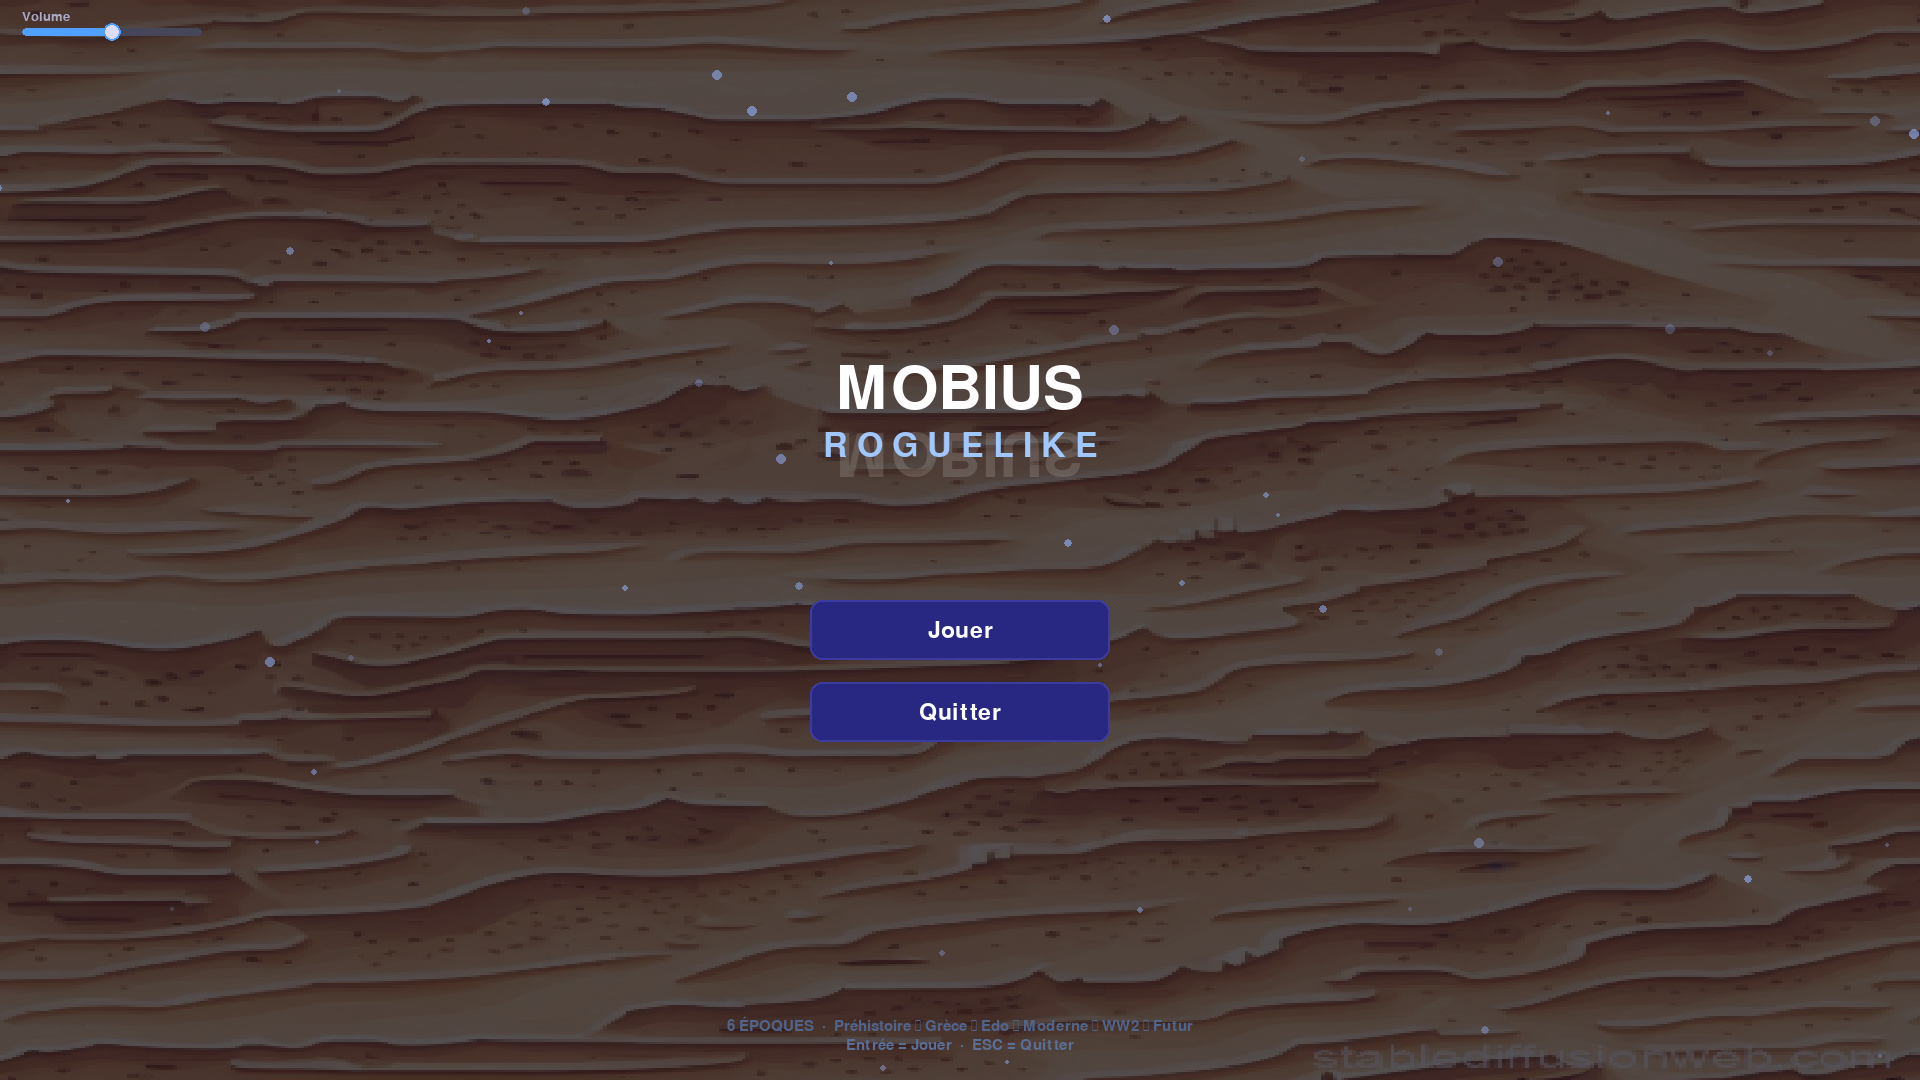
\includegraphics[width=0.8\textwidth]{images/menu-1.png}
  \caption{Annexe A1 \textemdash{} Menu principal}
\end{figure}

\begin{figure}[H]
  \centering
  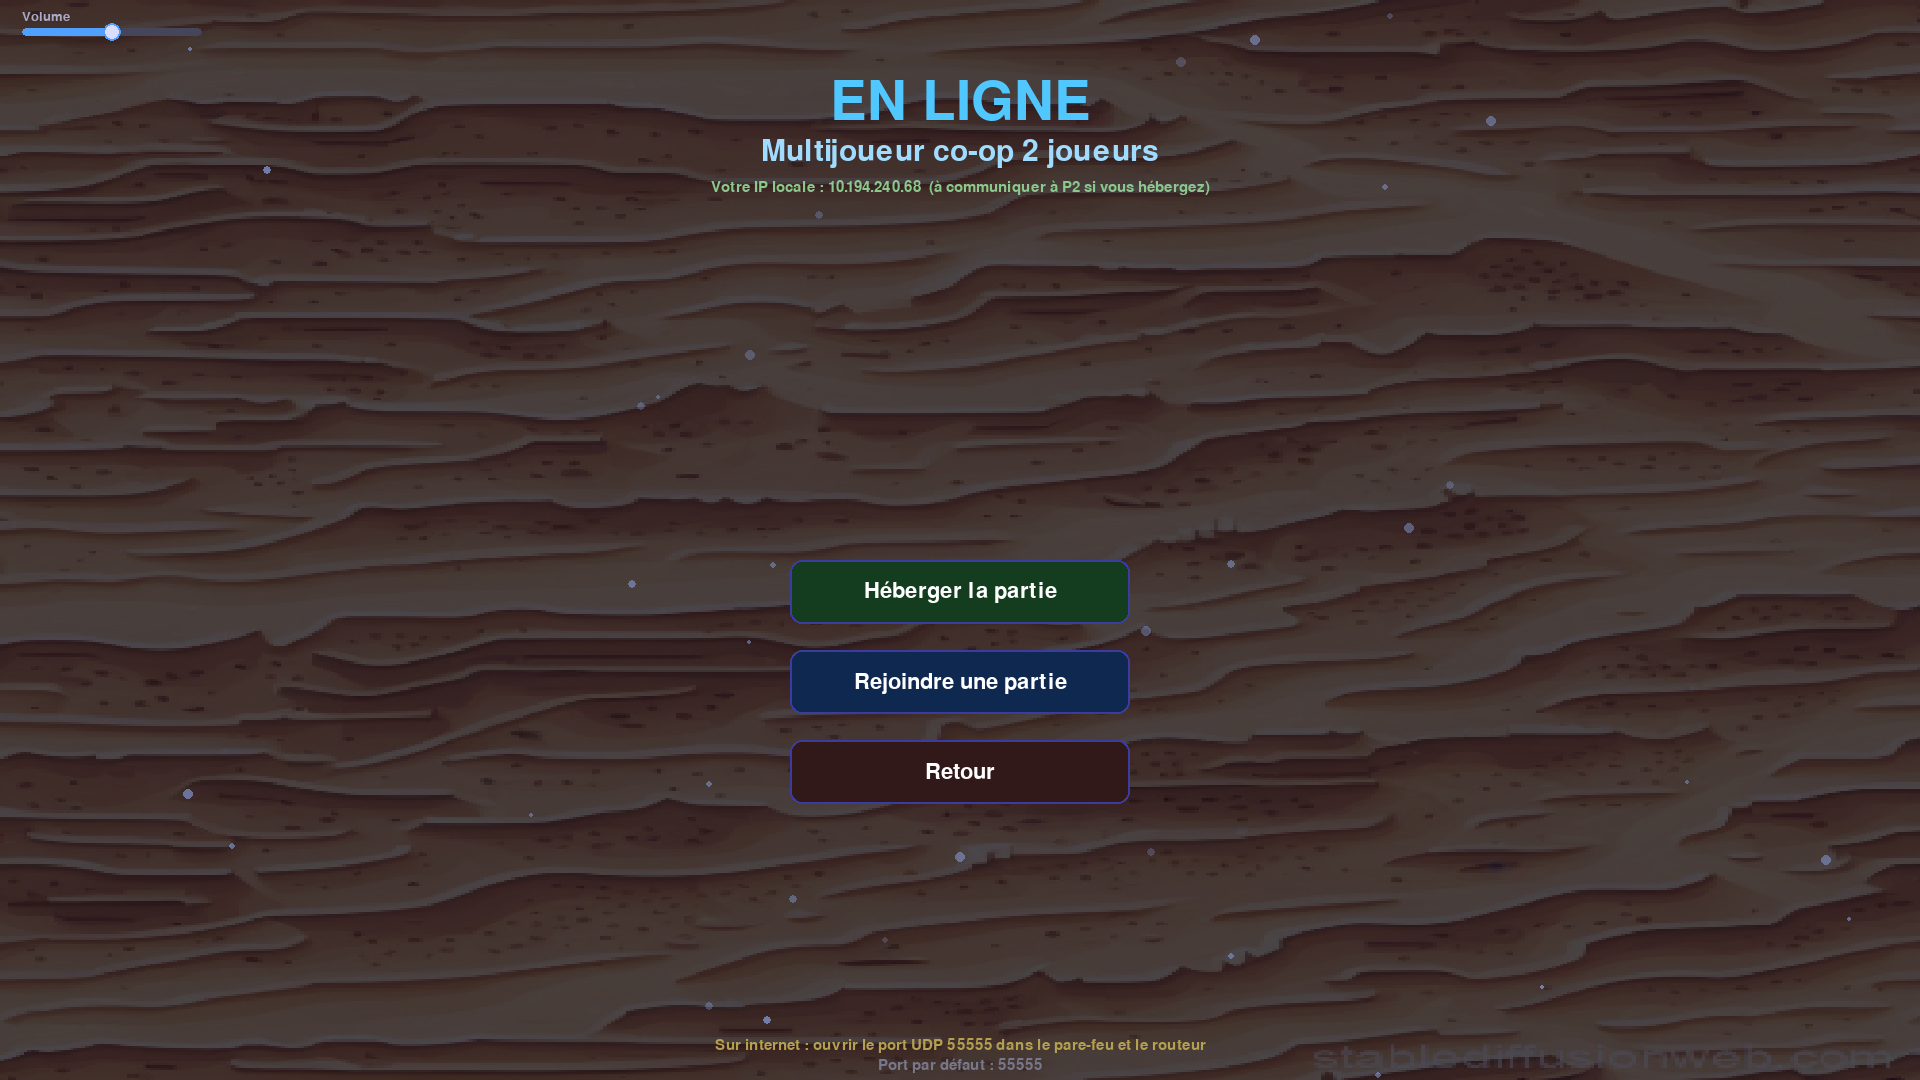
\includegraphics[width=0.8\textwidth]{images/multi.png}
  \caption{Annexe A2 \textemdash{} Sélection de mode}
\end{figure}

\begin{figure}[H]
  \centering
  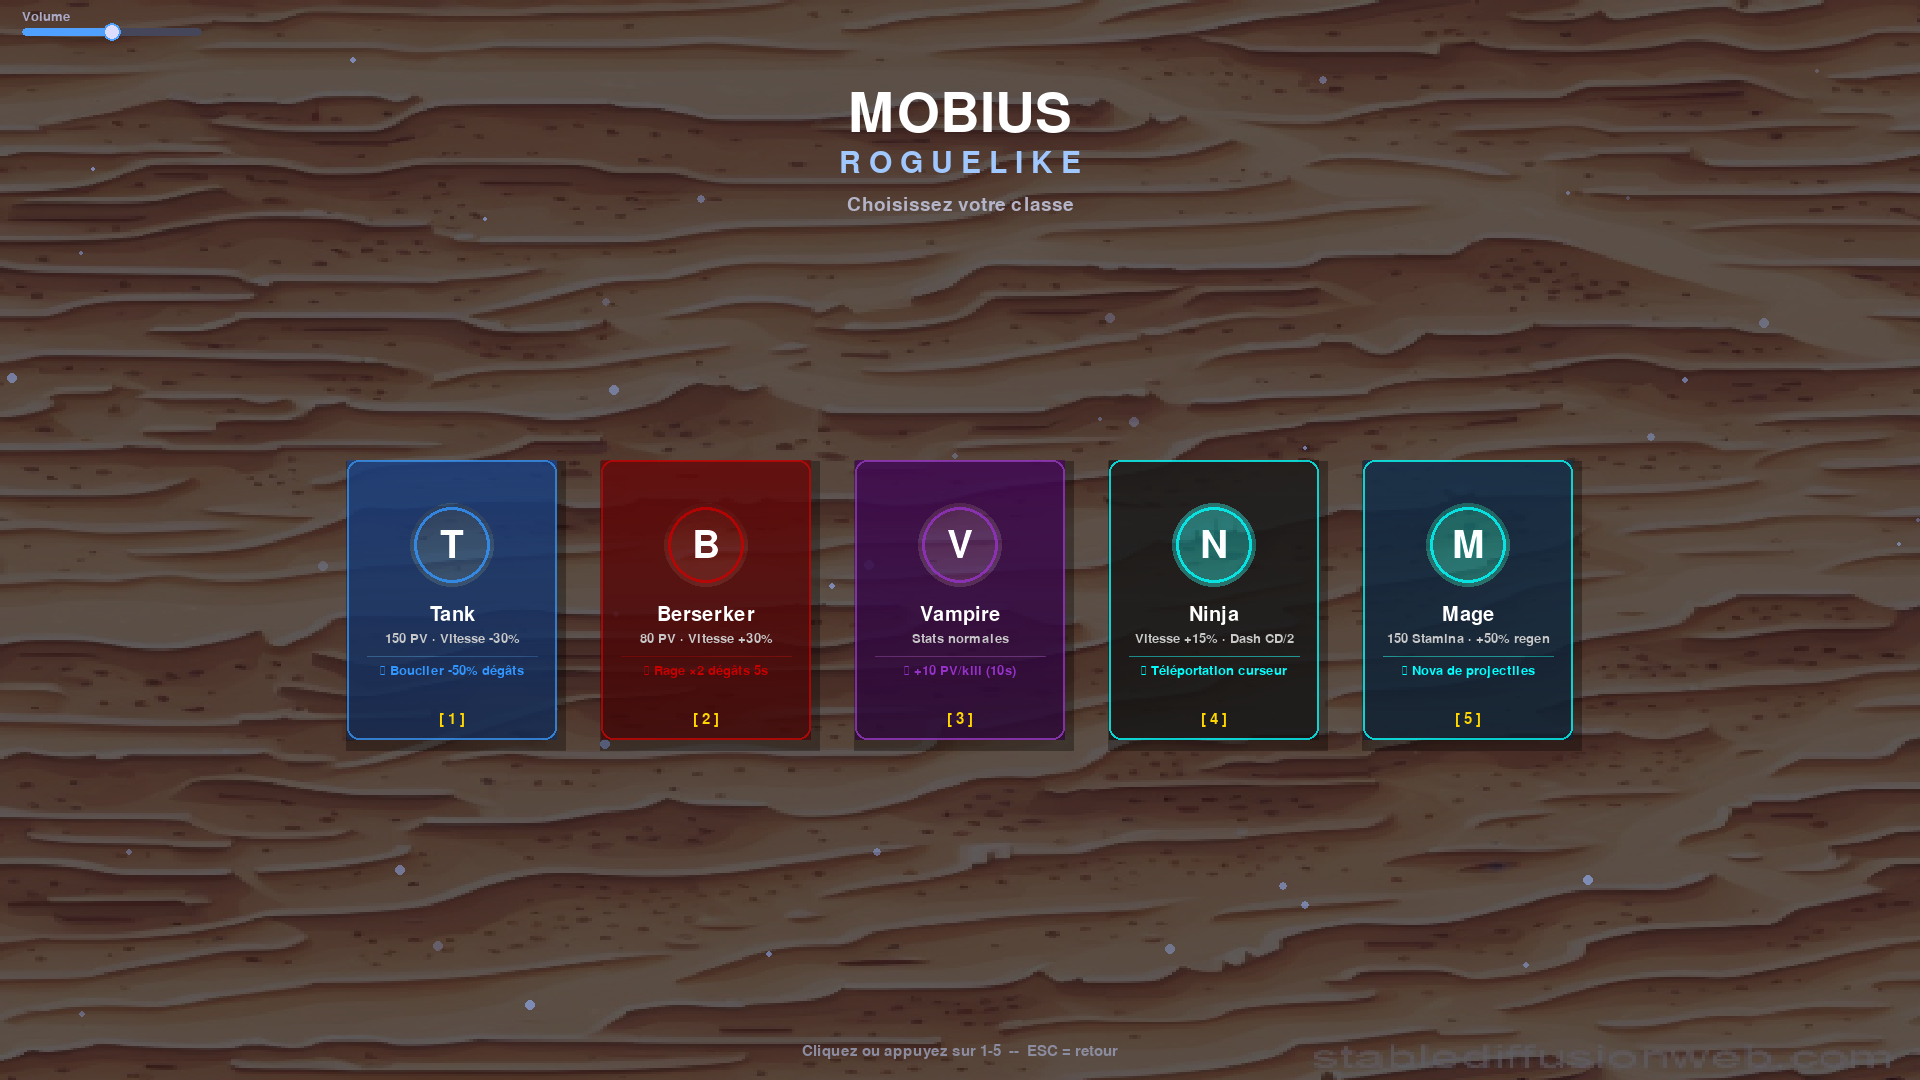
\includegraphics[width=0.8\textwidth]{images/choix-classes.png}
  \caption{Annexe A3 \textemdash{} Sélection de classe}
\end{figure}

\subsection{Gameplay \textemdash{} Époques}

\begin{figure}[H]
  \centering
  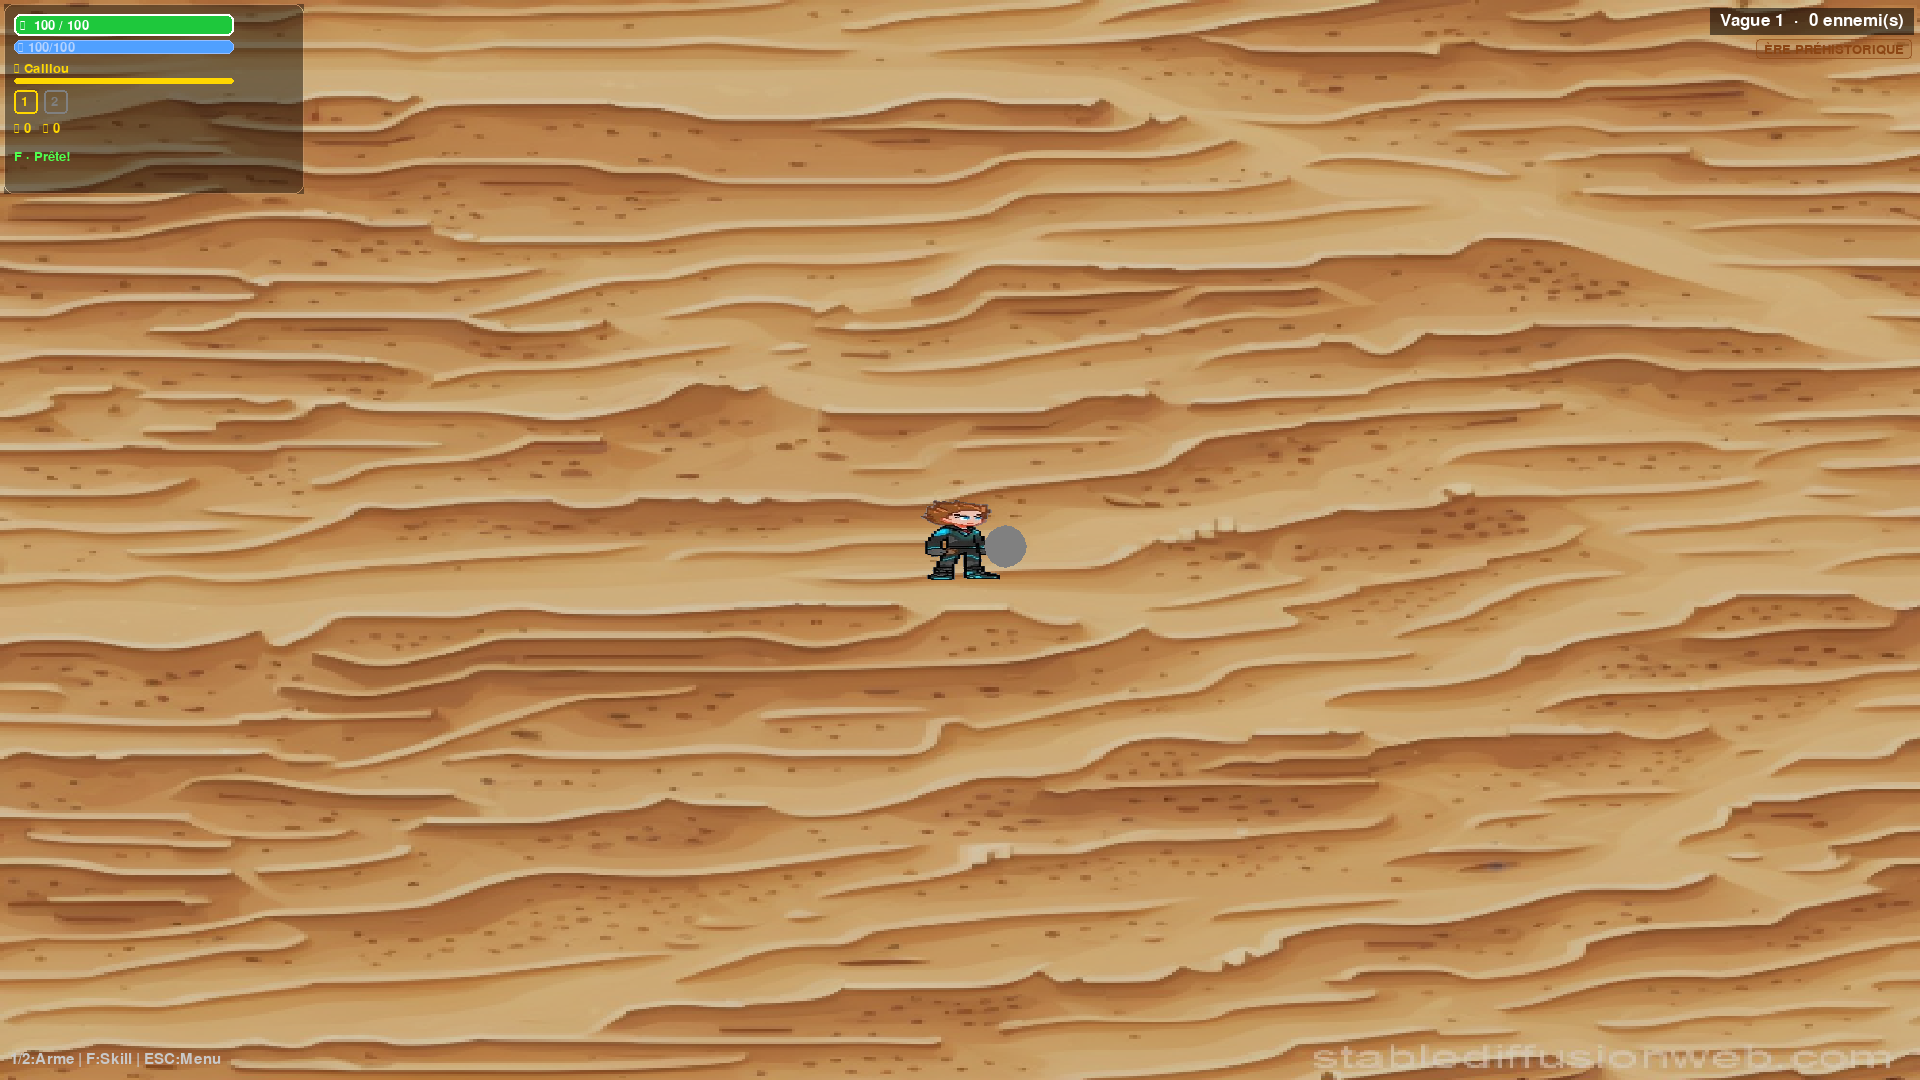
\includegraphics[width=0.8\textwidth]{images/prehistoire.png}
  \caption{Annexe B1 \textemdash{} Ère Préhistorique}
\end{figure}

\begin{figure}[H]
  \centering
  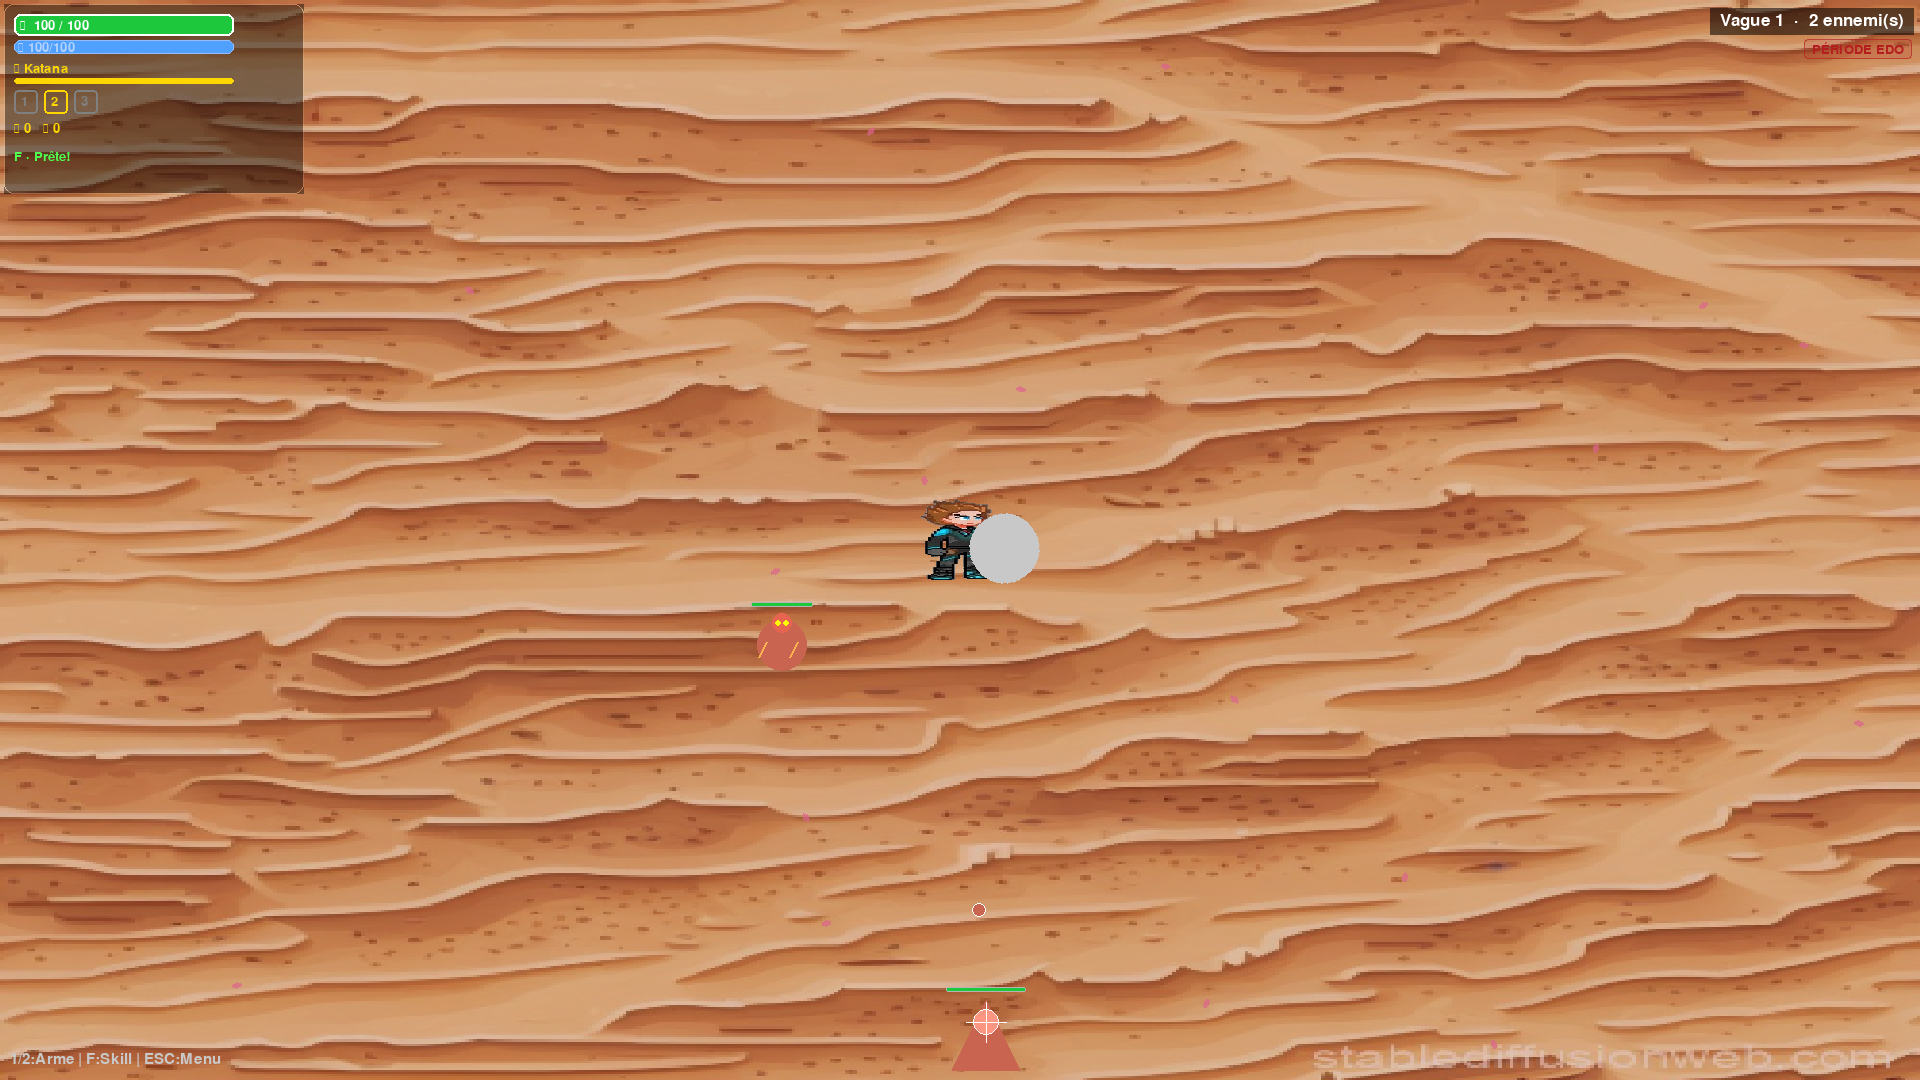
\includegraphics[width=0.8\textwidth]{images/edo.png}
  \caption{Annexe B2 \textemdash{} Période Edo}
\end{figure}

\begin{figure}[H]
  \centering
  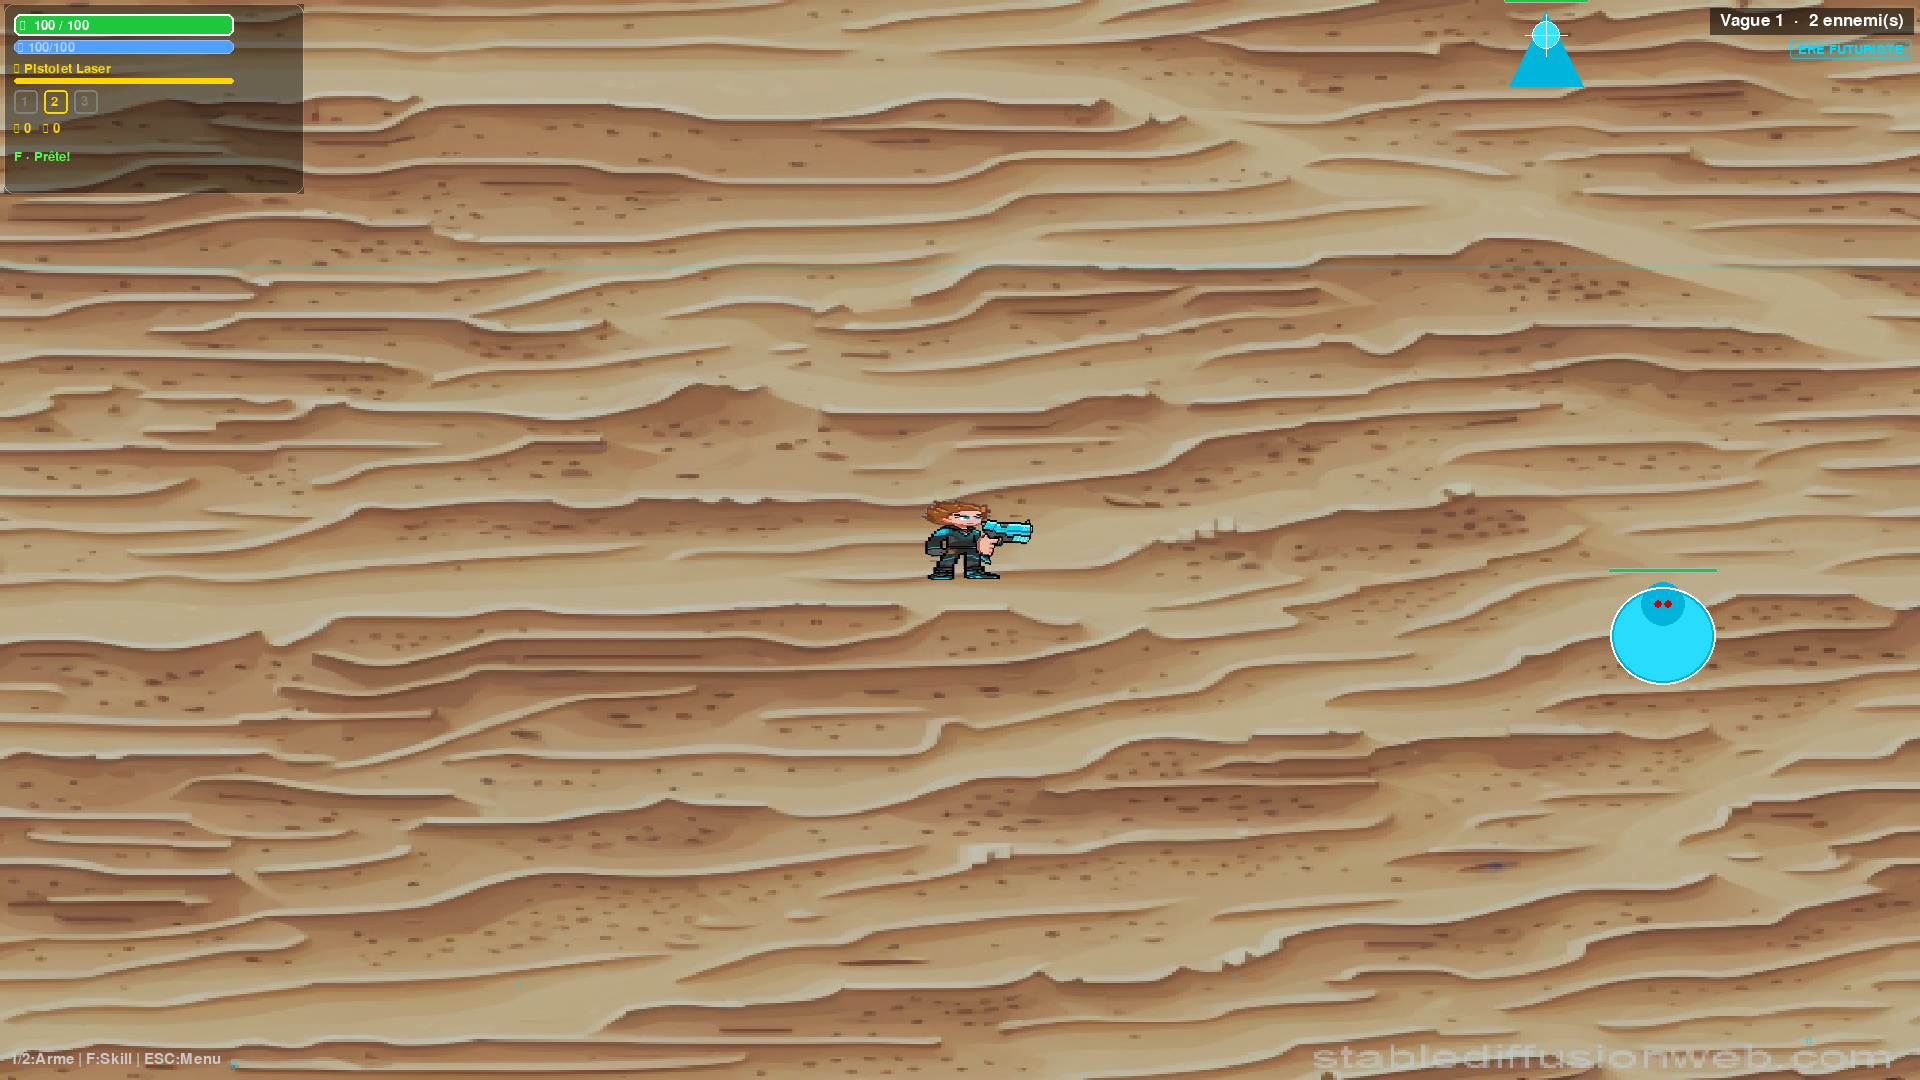
\includegraphics[width=0.8\textwidth]{images/futuristique.png}
  \caption{Annexe B3 \textemdash{} Ère Futuriste}
\end{figure}

\subsection{Multijoueur}

\begin{figure}[H]
  \centering
  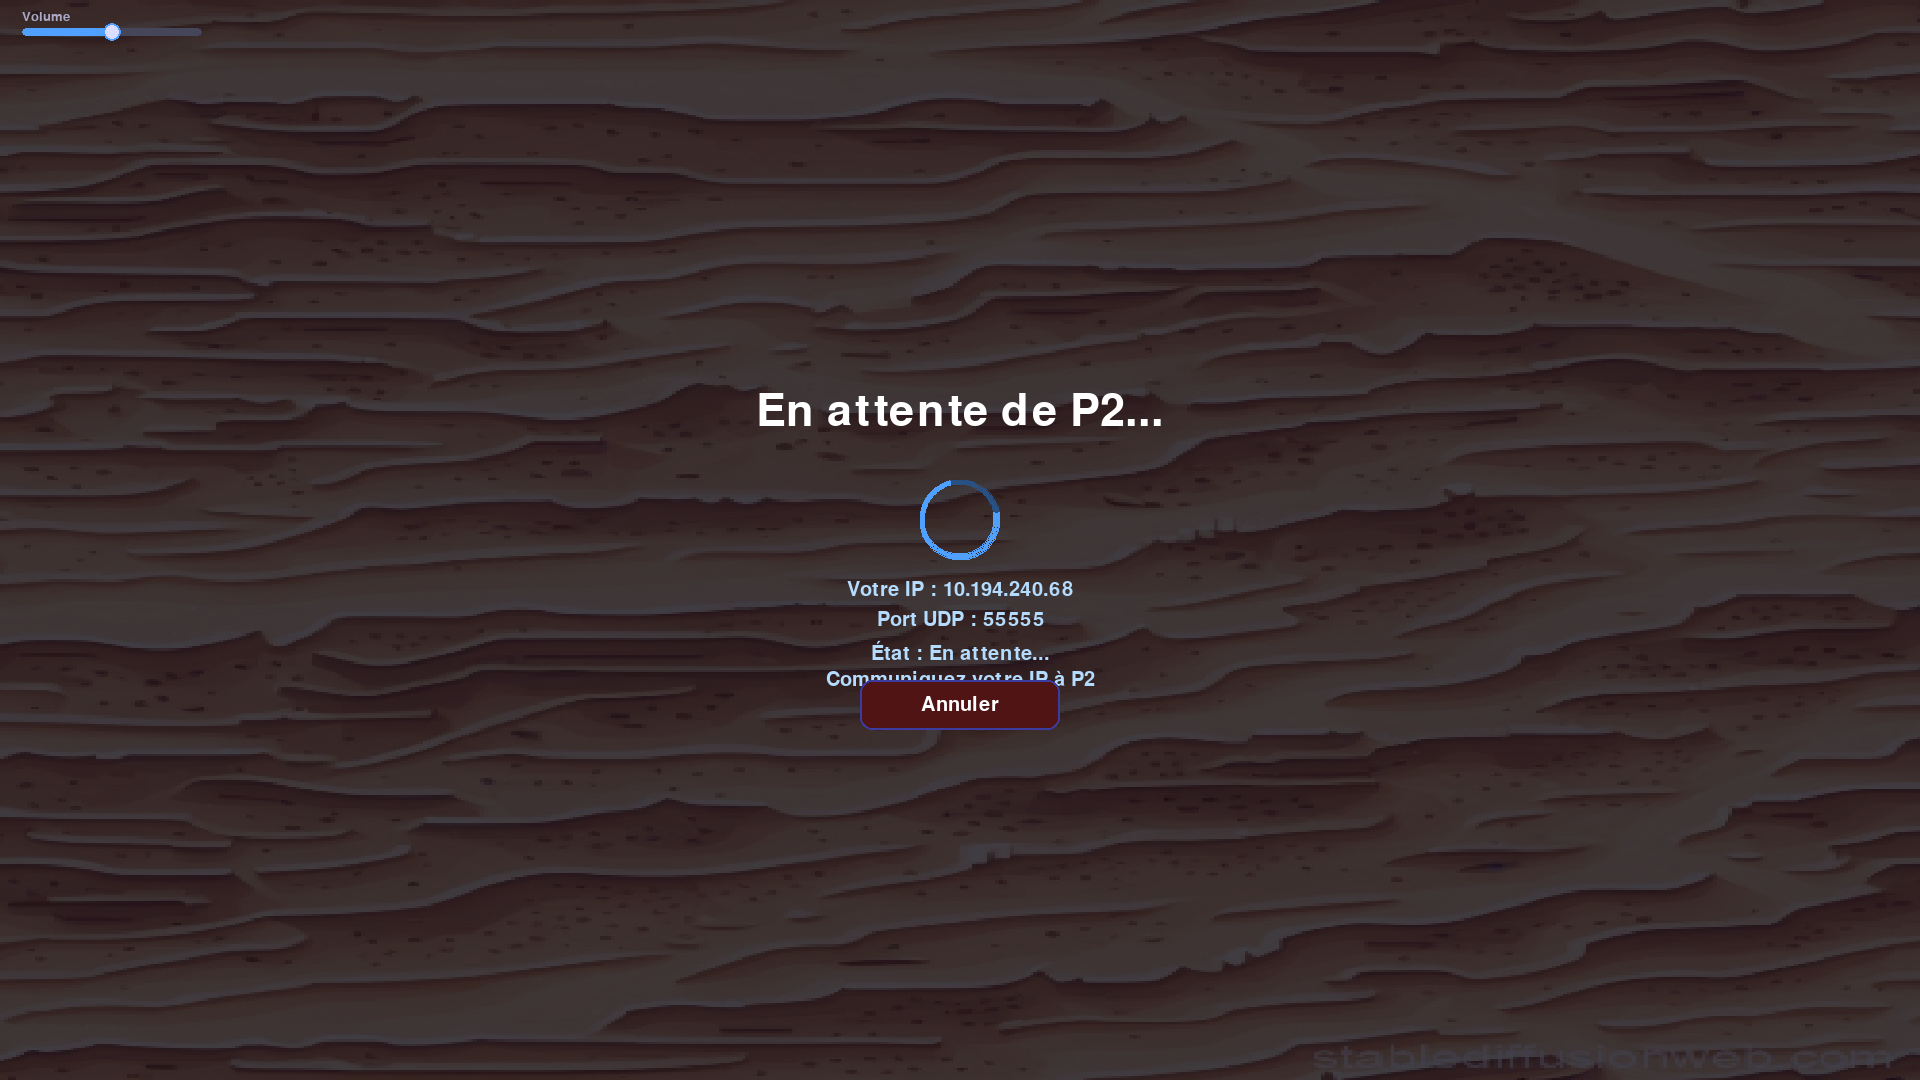
\includegraphics[width=0.8\textwidth]{images/host.png}
  \caption{Annexe C1 \textemdash{} Attente multijoueur (host)}
\end{figure}

\subsection{Communication \& planification}

\begin{figure}[H]
  \centering
  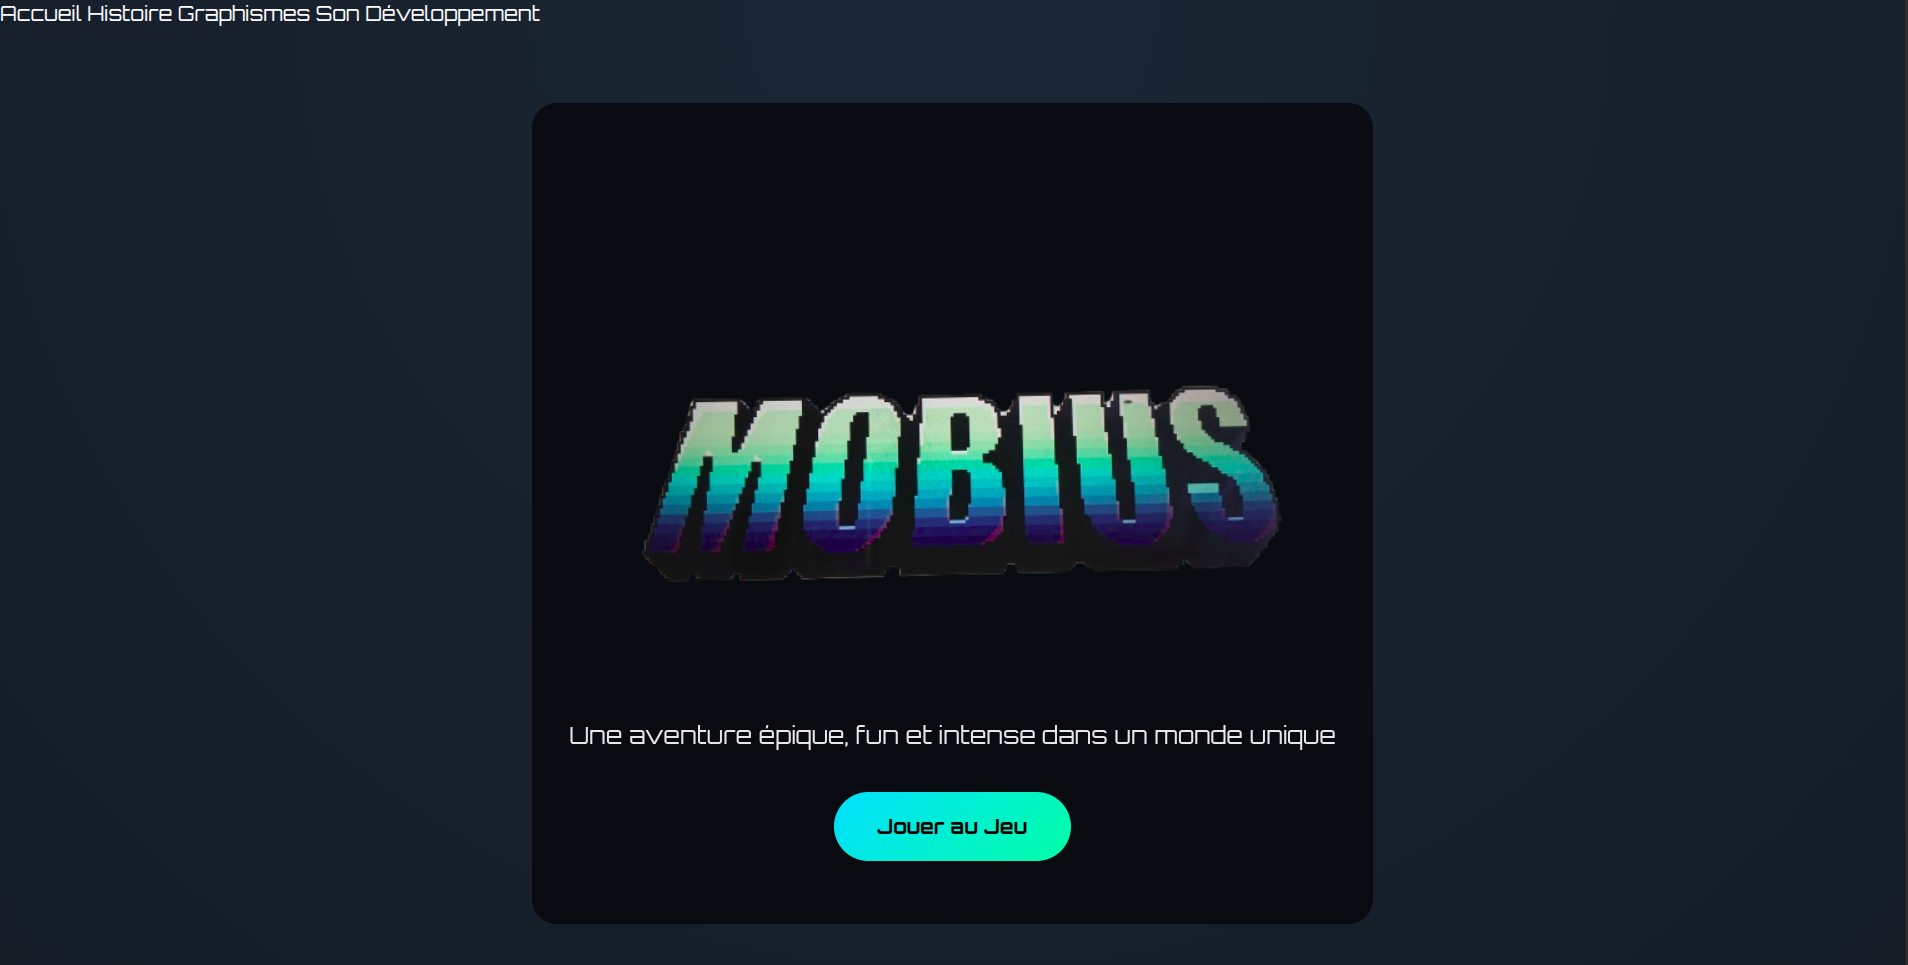
\includegraphics[width=0.8\textwidth]{images/site_web.png}
  \caption{Annexe D1 \textemdash{} Site web M3G\_STUDIO}
\end{figure}

% ─────────────────────────────────────────────────────────────
\section{Liens et ressources en ligne}
\label{ann:liens}

Cette annexe regroupe les liens vers les ressources accessibles en ligne pour compléter la présentation du projet.

\subsection*{Dépôt de code source}

\begin{tabular}{@{}ll@{}}
\textbf{GitHub M3G\_STUDIO} & \url{https://github.com/Epigold/Mobius_EPITA/} \\[3pt]
\end{tabular}


\bigskip
\noindent\textit{Note : les URLs ci-dessus sont les adresses prévues au moment de la soutenance. En cas d'indisponibilité, contacter directement l'équipe M3G\_STUDIO.}

\end{document}
